\documentclass[12pt,a4paper]{report}

%==============================================================================
% PACKAGE IMPORTS
%==============================================================================

% === Document Structure and Layout ===
\usepackage[utf8]{inputenc}           % For UTF-8 encoding
\usepackage{geometry}                 % For adjusting page layout and margins
\usepackage{fancyhdr}                 % For customizing page headers and footers
\usepackage{layout}                   % Use `\layout` to visualize the layout
\usepackage{titlesec}                 % For customizing section titles
\usepackage{float}                    % Positioning floating elements
\usepackage{tocloft}                  % For customizing the Table of Contents
\usepackage{setspace}                 % For line spacing
\usepackage{framed}                   % For framed environment

% === Mathematics, Symbols and Technical Content ===
\usepackage{amsmath}                  % Enhanced math typesetting
\usepackage{amssymb}                  % Additional math symbols
\usepackage{tikz-cd}                  % For commutative diagrams

% === Graphics, Figures and Diagrams ===
\usepackage{graphicx}                 % For graphics/images
\usepackage{tikz}                     % For vector graphics
\usepackage{tikz-3dplot}              % For 3D graphics

% === Tables and Arrays ===
\usepackage{array}                    % Enhanced tabular environments

% === Code Listings and Algorithms ===
\usepackage{algorithm}                % For algorithm blocks
\usepackage{algpseudocode}            % For pseudocode
\usepackage{listings}                 % For code listings
\usepackage{verbatim}                 % For multiline comments

% === Colors and Styling ===
\usepackage{xcolor}                   % Extended color support
\usepackage{color}                    % For color definitions
\usepackage[fitting]{tcolorbox}       % For colored boxes

% === References, Hyperlinks and Cross-Referencing ===
\usepackage{xurl}                     % For URLs
% \usepackage[
%     acronyms,       % For acronyms
%     acronym,        % For acronyms
%     automake,       % Automatically make glossaries
%     toc,            % Add glossaries to the Table of Contents
%     acronyms,       % Enable acronyms
%     nonumberlist    % Suppress page numbers in the glossary
% ]{glossaries}
% \makeglossaries                       % Initialize glossaries
\usepackage{bookmark}                 % Better PDF bookmarks (fixes warnings)
\usepackage{hyperref}                 % Enables hyperlinks and PDF metadata (bookmarks option removed)

% === Text Formatting and Typography ===
\usepackage[none]{hyphenat}           % Disables hyphenation throughout the document
\usepackage{pbox}                     % For parbox with line breaks
\usepackage{lmodern}                  % For Latin Modern needed for tcolorbox
\usepackage[T1]{fontenc}              % Use T1 font encoding for better character support
% \usepackage{textcomp}               % Provides \textquotedbl command
% \usepackage{mathptmx}               % Times New Roman font for math
% \usepackage{txfonts}                % Times New Roman font for text and math
\usepackage{times}                    % Times New Roman font for text
\renewcommand{\rmdefault}{ptm}      % Set Times New Roman as the default font


% === Miscellaneous Utilities ===
\usepackage{lipsum}                   % For placeholder text
\usepackage[nodayofweek]{datetime}    % For date formatting
\usepackage{etoolbox}                 % For patching commands
\usepackage{pgffor}                   % For loop constructs
\usepackage[useregional]{datetime2}

%==============================================================================
% STUDENT LIST MANAGEMENT
%==============================================================================
% This section provides commands for managing multiple students in group projects
% USAGE:
% 1. Add students using \addstudent{Student Name}{Roll Number} in the preamble
% 2. Use the various rendering commands in your document where needed
%
% Example usage:
%   \addstudent{John Doe}{CS21001}
%   \addstudent{Jane Smith}{CS21002}
%
% Then use in your document:
%   This project was completed by \studentgrammar.
%   OR
%   \begin{tabular}{|l|l|}\hline
%   Name & Roll Number \\\hline
%   \studenttable\hline
%   \end{tabular}
%   OR
%   \studentsignature
%
% CUSTOMIZATION:
% - Change text colors by modifying the \textcolor{red} and \textcolor{blue} values
% - Adjust spacing in \studentsignature with the \\[.8cm] value
% - Modify the formatting of names and roll numbers in each command as needed

\newcounter{studentcount}
\setcounter{studentcount}{-1}
\newcommand{\studentNamelist}{}    % Comma-separated list of student names
\newcommand{\studenttable}{}       % Table rows with names and roll numbers
\newcommand{\studentRolllist}{}    % List with names and roll numbers in parentheses
\newcommand{\studentlist}{}        % List of student names and roll numbers

% Main command to add a student to all lists
% Parameters: #1=Student Name, #2=Roll Number
\newcommand{\addstudent}[2]{%
    \updatestudentlist{#1}{#2}%
    \stepcounter{studentcount}
}

\newcommand{\updatestudentlist}[2]{%
    % Updates the student list and table with the new student
    % Parameters: #1=Student Name, #2=Roll Number
    % Adding to Student table
    \expandafter\gdef\expandafter\studenttable\expandafter{\studenttable \textcolor{blue}{\texttt{#1}} & \textcolor{blue}{\texttt{#2}}\\}

    \ifnum\value{studentcount}=-1
        % Adding to Student list for the first time
        \expandafter\def\expandafter\studentNamelist\expandafter{\studentNamelist \textcolor{red}{#1}}%
        % Adding to Student table
        \expandafter\gdef\expandafter\studentRolllist\expandafter{\studentRolllist {\textcolor{red}{#1}\- (\textcolor{red}{#2})}}%
        % Adding to Student list
        \expandafter\gdef\expandafter\studentlist\expandafter{\studentlist {{#1}/{#2}}}%
    \else
        % Adding to Student list for the subsequent time
        \expandafter\def\expandafter\studentNamelist\expandafter{\studentNamelist, \textcolor{red}{#1}}%
        % Adding to Student table
        \expandafter\gdef\expandafter\studentRolllist\expandafter{\studentRolllist, {\textcolor{red}{#1}\- (\textcolor{red}{#2})}}%
        % Adding to Student list
        \expandafter\gdef\expandafter\studentlist\expandafter{\studentlist, {{#1}/{#2}}}%
    \fi
}


% Creates a grammatically correct list with "and" before the last item
\newcommand{\studentgrammar}{%
    \foreach \n [count=\ni from 1] in \studentRolllist{%
        \n%
        \ifnum\ni=\value{studentcount} {and} \else\ifnum\ni<\value{studentcount}, \fi\fi%
    }%
}

% Creates a formatted signature block for all students
% Places two students per row by default
\newcommand{\studentsignature}{%
    % \vspace{0.2cm}  % Adjusts space between the signature block and the previous content
    \begin{center}
        % \par
        % \noindent\textbf{Signature}  % Uncomment to add "Signature" header
        % \par
        % \vspace{1cm}                 % Uncomment to add space after header
        \foreach \n [count=\ni from 1] in \studentNamelist{
            % Adds 2 students signature prompts in a row
            \ni. \n\ifodd\ni \hfil \else \\[.5cm] \fi
        }%
    \end{center}
    \vfill
    \vspace{-0.5cm}  % Adjusts space between signatures and the next content
}

\newcommand{\studentDeclareSign}{%
    \vspace{.5cm}  % Adjusts space between the signature block and the previous content
    \foreach \name/\roll in \studentlist {
        \begin{flushright}
            \textbf{\name} \\
            (Regd. No. \textbf{\texttt{\roll}})
        \end{flushright}
        \vspace{.5cm}  % Adjusts space between signatures and the next content
    }
}
%==============================================================================
% DOCUMENT VARIABLES
%==============================================================================
% IMPORTANT: Edit these variables to customize your document
% These variables are used throughout the document for titles, headers, etc.
% Changing them here will update them everywhere they are used

% --- Document Information ---
\newcommand{\docTitle}{Your Document Title - Title of the project}  % Full title of the document
\newcommand{\headerTitle}{Short Header Title}  % Use short title or \docTitle for header
\newcommand{\docSubtitle}{Subtitle (If Applicable)}
\newcommand{\batch}{XX}
\newcommand{\courseName}{Final Year Project}  % Course name (e.g., B.Tech, M.Tech, etc.)
\newcommand{\keyWords}{Keyword1, Keyword2, Keyword3}
\newcommand{\docVersion}{1.0}  % Document version

% --- Student Details ---
\newcommand{\studentName}{Student 1 Name}  % Full name of the student
\newcommand{\studentRoll}{217Y1A05XX}

\addstudent{\studentName}{\studentRoll}
% Use the \addstudent command to include additional students in the report.
% Example:
\addstudent{Student 2 Name}{217Y1A05YY}
% \addstudent{Student 3 Name}{217Y1A05ZZ}
% \addstudent{Student 4 Name}{217Y1A05AA}
% \addstudent{Student 5 Name}{217Y1A05BB}
% \addstudent{Student 6 Name}{217Y1A05CC}
% \addstudent{Student 7 Name}{217Y1A05DD}

% --- Institution Details ---
\newcommand{\college}{MLR Institute of Technology and Management}
\newcommand{\collegeShort}{MLRITM}
\newcommand{\collegeFull}{Marri Laxman Reddy Institute of Technology and Management, Hyderabad}
\newcommand{\university}{Jawaharlal Nehru Technological University, Hyderabad (JNTUH)}
\newcommand{\collegelogo}{MLRS-logo.png}
\newcommand{\collegebanner}{MLRS-banner.png}

% --- Department and Course Details ---
% Replace with your actual department and branch information
\newcommand{\deptName}{[Department Name]}                % Example: Department of Computer Science and Engineering
\newcommand{\deptNameShort}{[Dept. Short Name]}          % Example: Dept. of CSE
\newcommand{\branchName}{[Branch Name]}                  % Example: Computer Science and Engineering
\newcommand{\branchCode}{[Branch Code]}                  % Example: CSE or 05
\newcommand{\semester}{[Current Semester]}               % Example: VII (7th) Semester

% --- Guide and Faculty Details ---
% Replace placeholder text with actual names and titles
\newcommand{\guide}{[Guide Name]}                       % Example: Dr. S Pratap Singh
\newcommand{\guideDesignation}{[Position]}              % Example: Professor
\newcommand{\supervisor}{[Supervisor/Coordinator Name]}  % Example: Dr. S Pratap Singh
\newcommand{\supervisorDesignation}{[Supervisor Designation]}  % Example: Professor
\newcommand{\hod}{[HOD Name]}                           % Example: Dr. K. Abdul Basith
\newcommand{\hodDesignation}{Head of CSE Department}    % Example: Head of CSE Department
\newcommand{\principal}{[Principal Name]}               % Example: Dr. R. Murali Prasad
\newcommand{\principalDesignation}{Principal}           % Example: Principal
\newcommand{\director}{[Director Name]}                 % Example: Dr. P. Sridhar
\newcommand{\directorDesignation}{Director}             % Example: Director

% --- Academic Year ---
\newcommand{\academicYear}{2024--2025}  % Set the academic year

% --- Report Details ---
\newcommand{\reportType}{Major Project}

% --- Manual Date Option ---
% Custom date setting using datetime package
\newdate{customdate}{04}{04}{2024}  % Format: day, month, year
\renewcommand{\today}{\displaydate{customdate}}  % Make \today use our custom date
% The date will respect the defined formats like dashdate
% Also set the year to some other year if needed
% \renewcommand{\yearNum}{2023}  % Example: Set to 2023
\newcommand{\submissiondate}{\today}
\newcommand{\yearNum}{\the\year}
\newdateformat{dashdate}{\twodigit{\THEDAY}-\twodigit{\THEMONTH}-\THEYEAR}

% --- Metadata [Do not required editing] ---
\newcommand{\studentId}{\studentRoll}
\newcommand{\authorName}{\studentlist}
\newcommand{\authorID}{\studentId}

\newcommand{\pdfkeywords}{\keyWords}
\newcommand{\pdfauthor}{\studentRolllist}
\newcommand{\pdfsubject}{\courseName}
\newcommand{\reportName}{\reportType{} ({\academicYear})}

% Title page settings
\title{\docTitle}
\author{\authorName \\ \authorID \\ Guide: \guide}
\date{\today}  % Use \date{} for no date, or \date{Month Year} for a specific date

%==============================================================================
% CONFIGURATION SETTINGS
%==============================================================================
% These settings control the appearance and behavior of various document elements.
% Modify these settings to match your institution's requirements or your preferences.

% === TikZ and Graphics Configuration ===
\usetikzlibrary{external, shapes.geometric, arrows, arrows.meta, decorations.pathmorphing, calc}

% \usetikzlibrary{
%     arrows, arrows.meta, automata, backgrounds, calendar, 
%     chains, decorations, external, fadings, fit, 
%     matrix, patterns, patterns.meta, petri, 
%     positioning, scopes, shadows, shapes, 
%     shapes.geometric, shapes.arrows, shapes.symbols, 
%     shapes.misc, shapes.multipart, shapes.callouts,
%     spy, trees, turtle,
%     decorations.pathmorphing, decorations.pathreplacing, 
%     decorations.markings, decorations.footprints, 
%     decorations.shapes, decorations.text,
%     calc, fixedpointarithmetic, fpu, intersections, 
%     math, through,
%     3d, perspective,
%     circuits, circuits.logic, circuits.ee,
%     graphs, graphs.standard, 
%     er, folding, lindenmayersystems, 
%     mindmap, plothandlers, quotes, svg.path, topaths,
%     babel
% }
\graphicspath{{images/}{./}}          % Set paths for images - both in images/ folder and root directory

% === Color Definitions ===
% These colors are used throughout the document for various elements
% Modify them to match your institution's color scheme if necessary
\definecolor{bg}{HTML}{F2F2F2}                % Background color for code blocks
\definecolor{deepgray}{HTML}{666666}          % Dark gray
\definecolor{deepblue}{HTML}{000099}          % Dark blue
\definecolor{deepred}{HTML}{990000}           % Dark red
\definecolor{deepgreen}{HTML}{008000}         % Dark green
\definecolor{codegreen}{HTML}{009900}         % Green for comments
\definecolor{codegray}{HTML}{808080}          % Gray for line numbers
\definecolor{codepurple}{HTML}{9400D3}        % Purple for strings
\definecolor{backcolour}{HTML}{F2F2EC}        % Light background
\definecolor{brown}{HTML}{612322}             % Brown for headers/footers
\definecolor{darkred}{HTML}{C00000}          % Dark red for titles

% Project Report Title Styling
\newtcolorbox{titlebox}{
    colframe=white,             % Frame color white (invisible)
    colback=white,              % Background color white (invisible)
    boxrule=0pt,                % No border
    left=0pt,                   % No left padding
    right=0pt,                  % No right padding
    top=0pt,                    % No top padding
    bottom=0pt,                 % No bottom padding
    width=\textwidth,           % Full width of the text area
    fit to height=1in,          % Height of the box
    halign=center,              % Center the text horizontally
    valign=center,              % Center the text vertically
    fonttitle=\Huge\bfseries,   % Title font size and style
    fit basedim=26pt,           % Fit the box to the text height
    fontupper=\Huge\bfseries,   % Text font size and style
    coltitle=black,             % Title color
}

% === Code Listing Styles ===
\lstdefinestyle{pythonstyle}{
    keywords={False, await, else, import, pass, None, break, except, in, raise, True, class, finally, is, return, and, continue, for, lambda, try, as, def, from, nonlocal, while, assert, del, global, not, with, async, elif, if, or, yield}, % Python keywords
    keywordstyle=\color{deepblue}\bfseries,
    ndkeywords={self},
    ndkeywordstyle=\color{deepgray}\bfseries,
    identifierstyle=\color{black},
    sensitive=true,
    comment=[l]{\#},
    commentstyle=\color{deepgreen}\ttfamily,
    stringstyle=\color{deepred}\ttfamily,
    numberstyle=\tiny\color{gray},
    morestring=[b]',
    morestring=[b]``,
    basicstyle={
            \ttfamily
            \hyphenpenalty=50
            \exhyphenpenalty=50
            \linespread{1}\selectfont % Add \linespread{1}
        },
    breakatwhitespace=false,
    breaklines=true,
    captionpos=b,
    keepspaces=true,
    numbers=left,
    numbersep=5pt,
    showspaces=false,
    showstringspaces=false,
    showtabs=false,
    tabsize=2
}

\lstdefinelanguage{JavaScript}{
    keywords={break, case, catch, continue, debugger, default, delete, do, else, false, finally, for, function, if, in, instanceof, new, null, return, switch, this, throw, true, try, typeof, var, void, while, with, let, const},
    sensitive=true,
    comment=[l]{//},
    morecomment=[s]{/*}{*/},
    morestring=[b]",
    morestring=[b]'
}

\lstdefinestyle{graystyle}{
    backgroundcolor=\color{backcolour},
    commentstyle=\color{codegreen},
    keywordstyle=\color{magenta},
    numberstyle=\tiny\color{codegray},
    stringstyle=\color{codepurple},
    basicstyle={\ttfamily\hyphenpenalty=50\exhyphenpenalty=50\linespread{1}\selectfont}, % Add \linespread{1}
    comment=[l]{\#},
    commentstyle=\color{deepgreen}\footnotesize\rmfamily,
    breakatwhitespace=false,
    breaklines=true,
    captionpos=b,
    keepspaces=true,
    numbers=left,
    numbersep=5pt,
    showspaces=false,
    showstringspaces=false,
    showtabs=false,
    tabsize=2
}

\lstset{style=graystyle}

% captions settinng
\captionsetup[listing]{
    font=small, % Set font size for captions
    labelformat=simple, % Use simple label format
    labelfont=normalfont,
    textfont={bf, tt},
}

% Configure listing settings for minted
% \usemintedstyle{friendly}
% \usemintedstyle{borland}
\setminted{
    linenos=true,
    numbersep=5pt,
    frame=none,
    tabsize=2,
    breaklines=true,
    breakanywhere=true,
    autogobble=true,
    baselinestretch=1, % Set line spacing for minted
}

% Configure minted, listings, and algorithm environments
% Synchronize the `listing` counter with `lstlisting`
\AtBeginEnvironment{listing}{\refstepcounter{lstlisting}}
\renewcommand{\thelisting}{\thechapter.\arabic{lstlisting}}
\renewcommand{\theFancyVerbLine}{\normalfont\tiny\color{gray}\arabic{FancyVerbLine}} % Customize line number style
\newenvironment{longlisting}{\captionsetup{type=listing}}{}

% Set page geometry with 1-inch margins on A4 paper
\geometry{margin=1in}  % Uncomment to set 1-inch margins

% Configure hyperref for proper cross-references and bookmarks
\hypersetup{
    breaklinks=true,            % allow line breaks in links
    pdfstartview={FitH},        % fits the width of the page to the window
    pdftitle={\docTitle},       % title
    pdfauthor={\pdfauthor},     % author
    pdfsubject={\pdfsubject},   % subject of the document
    pdfcreator={\studentlist},  % creator of the document
    pdfkeywords={\pdfkeywords}, % list of keywords
    colorlinks=false,           % false: boxed links; true: colored links
    linkcolor=deepblue,         % color of internal links
    citecolor=deepred,          % color of links to bibliography
    filecolor=deepgreen,        % color of file links
    urlcolor=blue               % color of external links
}

% Typography settings
\sloppy
\hfuzz=99pt                     % Suppress warnings for overfull hboxes
\vfuzz=99pt                     % Suppress warnings for overfull vboxes
\hbadness=10000                 % Suppress warnings for underfull hboxes
\exhyphenpenalty=10000          % Suppress hyphenation across lines
\hyphenpenalty=10000            % Suppress hyphenation across lines
% \raggedbottom                   % Allow pages to be ragged at the bottom

\renewcommand{\cftbeforetoctitleskip}{-.5em}
% \renewcommand{\cftaftertoctitleskip}{1em}
\renewcommand{\contentsname}{\hfil Contents}
\addtocontents{toc}{
    \textbf{S .No. \leftskip2cm Chapter Name \hfill Page No.}\par
}   % Add 'S. No.', 'Name of Chapter', and 'Page No.' to the ToC

% Add a horizontal line after the Table of Contents header
\addtocontents{toc}{
    \protect\mbox{}\protect\hrulefill\par
}% Add a horizontal line after the ToC header

% %==============================================================================
% % ACRONYM DEFINITIONS
% %==============================================================================
% % Define acronyms that will be used throughout the document
% % Format: \newacronym{label}{abbreviation}{full form}
% \newacronym{ai}{AI}{Artificial Intelligence}
% \newacronym{ml}{ML}{Machine Learning}
% \newacronym{nlp}{NLP}{Natural Language Processing}


% %===============================================================================
% % ADDITIONAL SETTINGS
% %===============================================================================
% % Add any additional settings or configurations here
% % Chpater Tittle Formatting
% \titleformat{\chapter}[display]
%     {\normalfont\huge\bfseries\raggedleft}
%     {\vspace{-40pt}                                 % Space before chapter number
%     \chaptertitlename\ \thechapter}
%     {5pt}                                           % Reduced space between chapter number and title
%     {\Huge}                                         % Title font size
%     []                                              % No additional code after title


\begin{document}
   % --- Main Content ---
\chapter{Introduction}
\label{chap:introduction}

The introduction should provide background information on your topic, explain the significance of your research, and clearly state your research question or objective. This chapter should also outline the structure of the document and briefly summarize each subsequent chapter. 
\section{Background}
This section should provide context for your research, explaining fundamental concepts necessary for understanding your work. 
% Artificial Intelligence (\gls{ai}) is a rapidly growing field. Subfields such as \gls{ml} and \gls{nlp} are gaining significant attention.

\section{Motivation}
Explain why your research topic is important and what gap in knowledge it addresses.

\section{Problem Statement}
Clearly articulate the specific problem or question your research aims to address.

\section{Outline of the Report}
Provide a brief overview of the structure of your document, summarizing the content of each chapter.

% CHAPTER 2: LITERATURE REVIEW
\chapter{Literature Review}
This chapter should synthesize existing research relevant to your topic. Analyze the current state of knowledge, identify gaps, and position your research within the existing literature.

\section{Overview of Existing Work}
Summarize key research papers, books, and other sources related to your topic.

\section{Current Trends}
Discuss recent developments and emerging trends in your research area.

\section{Research Gaps}
Identify limitations or gaps in existing research that your work aims to address.

% --- Theoretical Framework ---
% CHAPTER 3: THEORETICAL FRAMEWORK
\chapter{Theoretical Framework}
Present the theoretical foundation of your research, including relevant models, equations, algorithms, or principles.

\section{Key Concepts}
Define and explain the fundamental concepts central to your research.

\section{Mathematical Formulation}
Present any relevant mathematical formulations, theorems, or proofs.

\section{Algorithms}
This section presents the algorithms used in this research.

% Example of how to include an algorithm with proper referencing
Algorithm \ref{alg:example} demonstrates a basic search algorithm. This example shows how to properly format and include algorithms in your document.

\begin{algorithm}
\caption{Binary Search Algorithm}
\label{alg:example}
\begin{algorithmic}[1]
\Procedure{BinarySearch}{$A, n, x$}
    \State $low \gets 1$
    \State $high \gets n$
    \While{$low \leq high$}
        \State $mid \gets low + \lfloor (high - low) / 2 \rfloor$ \Comment{Avoid integer overflow}
        \If{$A[mid] < x$}
            \State $low \gets mid + 1$
        \ElsIf{$A[mid] > x$}
            \State $high \gets mid - 1$
        \Else
            \State \Return $mid$
        \EndIf
    \EndWhile
    \State \Return $-1$
\EndProcedure
\end{algorithmic}
\end{algorithm}

\subsection{Algorithm Complexity Analysis}
When analyzing the time complexity of Algorithm \ref{alg:example}, we find that binary search operates in $O(\log n)$ time, where $n$ is the number of elements in the sorted array. This is because each comparison eliminates approximately half of the remaining elements.

\subsection{Pseudocode Formatting Tips}
When writing algorithms:
\begin{itemize}
    \item Use consistent indentation
    \item Number each line for easy reference with \texttt{algorithmic[1]}
    \item Include proper comments for complex steps
    \item Clearly define inputs and outputs of procedures
\end{itemize}

% IMPORTANT: Always reference every figure in the text BEFORE it appears
Figure \ref{fig:external_image} illustrates a key concept of this research. As shown in the figure, important relationships between variables can be visualized.
As shown in Figure \ref{fig:tikz_figure}, the following diagram illustrates the relationship between key variables.

% Example of adding a referenced figure
\begin{figure}[H]
    \centering
    \includegraphics[width=0.5\textwidth]{example-image.jpg} % Replace 'sample-figure.jpg' with your image file name
    \caption[Short caption for sample figure]{Detailed caption explaining the sample figure. The short caption appears in the list of figures.}
    \label{fig:external_image}
\end{figure}

% Example of drawing a figure using TikZ
\begin{figure}[H]
    \centering
    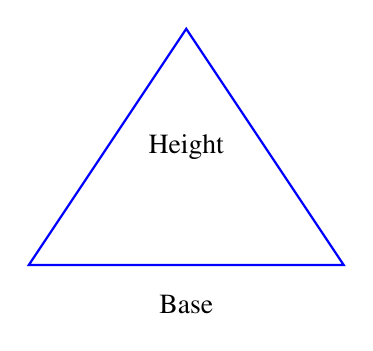
\begin{tikzpicture}
        % Example TikZ drawing: A simple triangle
        \draw[thick, blue] (0,0) -- (4,0) -- (2,3) -- cycle;
        \node at (2,-0.5) {Base};
        \node at (2,1.5) {Height};
    \end{tikzpicture}
    \caption[Short caption for TikZ figure]{Detailed caption explaining the TikZ-drawn figure. The short caption appears in the list of figures.}
    \label{fig:tikz_figure}
\end{figure}

% IMPORTANT: Every figure must be referenced in the text (e.g., "As shown in Figure \ref{fig:label}...")

\section{Example Implementation}
Listing \ref{lst:python_example} demonstrates a Python function implementation that doubles its input parameter. This code sample illustrates how to include formatted code in your document with syntax highlighting.

\begin{lstlisting}[language=Python, caption=Example Python Code, breaklines=true, label=lst:python_example]
def example_function(parameter):
    """
    This is a sample function to demonstrate code inclusion. It takes a parameter and returns its double.
    :param parameter: The input value to be doubled.
    """
    result = parameter * 2
    return result

# Example usage
value = 42
print(f"The result is: {example_function(value)}")
\end{lstlisting}

\subsection{Example Equations}
Below are sample equations formatted in LaTeX:

% Inline equation example
The quadratic formula $ax^2 + bx + c = 0$ has the solution $x = \frac{-b \pm \sqrt{b^2 - 4ac}}{2a}$.

% Display equation example
\begin{equation}
    E = mc^2
\end{equation}

% Equation array example
\begin{align}
    (a+b)^2 &= a^2 + 2ab + b^2\\
    (a-b)^2 &= a^2 - 2ab + b^2
\end{align}

% --- Methodology ---
% CHAPTER 4: METHODOLOGY
\chapter{Methodology}
Describe your research approach, methods, experimental setup, and data collection procedures.

\section{Research Approach}
Explain the overall approach or strategy you used in your research.

\section{Experimental Setup}
Describe the equipment, materials, or software used in your research.

\section{Data Collection}
Explain how you collected data, including any sampling strategies or selection criteria.

\section{Analysis Methods}
Describe the statistical techniques or analytical methods you used to process and interpret your data.

% --- Results and Discussion ---
% CHAPTER 5: RESULTS AND DISCUSSION
\chapter{Results and Discussion}
Present your findings and interpret them in the context of your research question and existing literature.

\section{Key Findings}
Describe the main results of your research, supported by data, figures, or tables.

% IMPORTANT: Notice that the table is referenced in the text BEFORE it appears
% Always reference tables in your text before they are displayed
Table \ref{tab:sample_table} presents the sample data collected during the experiment.

\begin{table}[ht]
    \centering
    \caption{Sample Table Format}  % Table caption
    \label{tab:sample_table}       % Label for referencing the table in text
    \begin{tabular}{|l|c|r|}       % l=left-aligned, c=centered, r=right-aligned columns
        \hline
        \textbf{Column 1} & \textbf{Column 2} & \textbf{Column 3} \\
        \hline
        Row 1, Cell 1 & Row 1, Cell 2 & Row 1, Cell 3 \\
        Row 2, Cell 1 & Row 2, Cell 2 & Row 2, Cell 3 \\
        Row 3, Cell 1 & Row 3, Cell 2 & Row 3, Cell 3 \\
        \hline
    \end{tabular}
\end{table}

\section{Discussion}
Interpret your findings, explain their significance, and discuss how they relate to existing research.

\section{Limitations}
Acknowledge any limitations or constraints in your research methodology or findings.

% --- Conclusion ---
% CHAPTER 6: CONCLUSION
\chapter{Conclusion and Future Work}
Summarize the key findings, contributions, and implications of your research, and suggest directions for future investigation.

\section{Summary of Contributions}
Highlight the main contributions or advancements your research has made to the field.

\section{Future Research Directions}
Propose potential areas for future research that build upon your findings or address limitations.

\section{Final Remarks}
Offer final insights or reflections on the significance of your research.
% Include citations in the document
As discussed in \cite{Sample2023}, the topic is highly relevant. Refer to \cite{Book2022} for more details.

\begin{thebibliography}{99}
    % Sample bibliography entries - REPLACE WITH YOUR REFERENCES
    % Format for journal articles:
    \bibitem{Sample2023}
    Author, A., \& Co-Author, B. (2023). 
    \textit{Title of the article or paper}. 
    Journal Name, Volume(Issue), Page range. 
    \href{https://doi.org/10.1000/sample}{https://doi.org/10.1000/sample}
    
    % Format for books:
    \bibitem{Book2022}
    Author, C. (2022). 
    \textit{Title of the Book}. 
    Publisher Name.
    
    % Format for websites:
    \bibitem{Website2023}
    Organization Name. (2023). 
    \textit{Title of the webpage}. 
    Retrieved Month Day, Year, from \url{https://www.example.com/page}
\end{thebibliography}
\end{document}